% !TeX TXS-program:compile = txs:///pdflatex/[--shell-escape]

\documentclass[11pt, letterpaper]{article}

\usepackage{minted}
\usepackage[utf8]{inputenc}
\usepackage[T1]{fontenc}
\usepackage{lmodern}
\usepackage{graphicx}
\usepackage{longtable}
\usepackage{wrapfig}
\usepackage{rotating}
\usepackage{amsmath}
\usepackage{textcomp}
\usepackage{amssymb}
\usepackage{hyperref}
\usepackage[round]{natbib}
\usepackage{subcaption}


\title{\bfseries Tarea}
\author{Ángel García Báez}
\date{\today}
\setcounter{tocdepth}{3} 

\begin{document}
	
	% Página de presentación
	\begin{titlepage}
		\centering
		
\includegraphics[width=0.2\textwidth]{logo.png}\par
		\vspace{1cm}
		{\LARGE \bfseries Universidad Veracruzana \par}
		\vspace{1cm}
		{\Large Maestría en Inteligencia Artificial\par}
		\vspace{3cm}
		{\LARGE \bfseries Visión por Computadora \par}
		\vspace{1cm}
		{\Large \bfseries Tarea 12. Clasificación binaria de imagenes de gusanos mediante una red neuronal convolucional en MATLAB \par}
		\vfill
		{\Large \textit{Ángel García Báez}\par}
		\vspace{1cm}
		{\Large Profesor: Dr. Héctor Acosta Mesa \par}
		\vfill
		{\Large \today \par}
	\end{titlepage}
	
	% Página exclusiva para la tabla de contenidos
	\newpage
	\tableofcontents
	\newpage
	
% Sección para el problema 1
\section{Objetivo de la práctica}

Para la presente practica, se cuenta con un conjunto de 93 imágenes en formato .tif de gusanos, de los cuales 48 están etiquetados como "vivos" y 45 están identificados como muertos. A continuación se muestra una muestra de como son estas imágenes.


\begin{figure}[h!]
	\centering
	\begin{minipage}{0.8\textwidth}
		\centering
		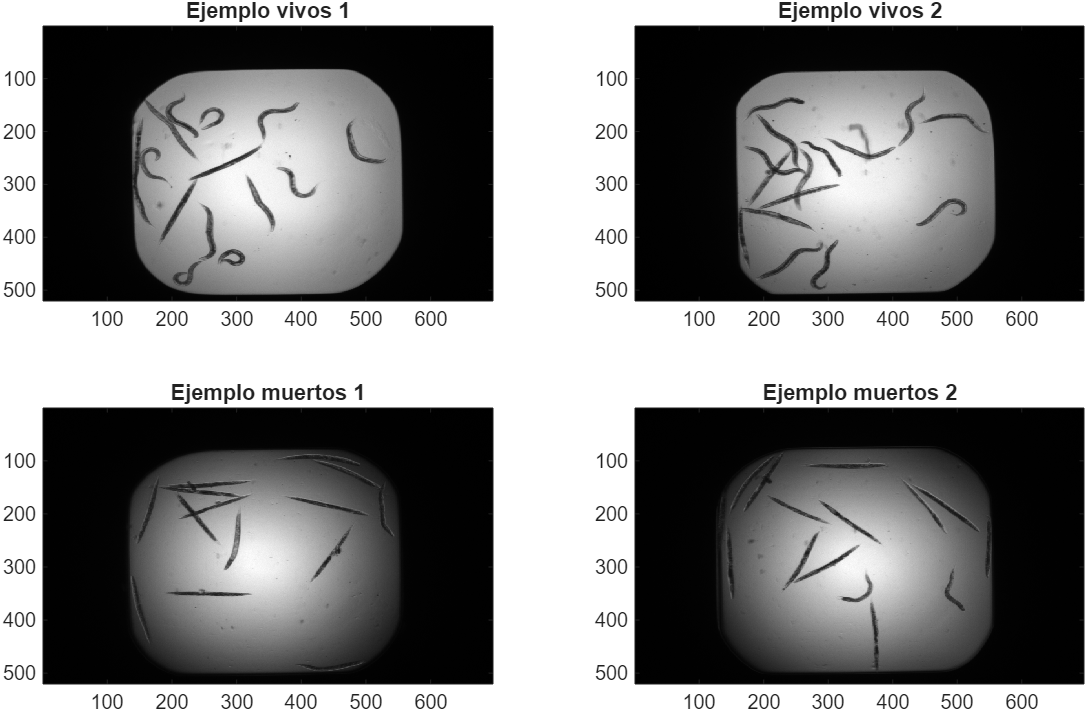
\includegraphics[width=\textwidth]{IMG/R1.png}
		\caption*{Muestra de gusanos vivos y muertos.}
	\end{minipage}\hfill
\end{figure}

Se observan claras diferencias entre el comportamiento de ambas imagenes, para el caso de los gusanos vivos, se percibe movimientos y formas curvas. Para el caso de los gusanos muertos, se perciben en posiciones rectas. \\

Una vez entendido esto, lo que se pide hacer es lo siguiente:


\begin{itemize}
	\item Se pide implementar una metodología usando redes neuronales convolucionales para llevar a cabo la clasificación binaria (vivos o muertos) de las imágenes.
	
	\item Se espera lograr un minimo de buena clasificación del 90\%
	
\end{itemize}




	
\newpage
	
\section{Metodología}

\subsection{Modelo estadístico de forma usando PCA}

A continuación se describe el proceso de modelado estadístico de forma conforme a lo explicado en \cite{MPHY0026_SSM}, \cite{SSM_PCA_Basel}, \cite{cootes_pdms} y \cite{sarkalkan_statistical_2014} que retoman la idea del PCA vista en \cite{johnson2007} pero con los resultados de haber hecho el proceso de registro como se explica en \cite{coste2012image}.

Para cada rostro, se tiene un conjunto de puntos (20 observaciones) que representan los puntos claves utilizados para el proceso de registro, esto equivale a tener una matriz de datos de tamaño $20 \times 2$ por cada una de las imágenes que se ve así:


$$
\mathbf{x}^{(i)} = 
\begin{bmatrix} 
	x_1 & y_1 \\
	x_2 & y_2 \\
	\vdots & \vdots \\ 
	x_{20} & y_20 
\end{bmatrix} 
$$

Ahora, cada uno de esa pareja de puntos va a ser concatenada como un solo vector fila tal y como se muestra a continuación:

$$
\mathbf{x}^{(i)} = \begin{bmatrix} x_1 & y_1 & x_2 & y_2 & \cdots & x_n & y_n \end{bmatrix}
$$

Posteriormente, se construye una nueva matriz $X$ de forma que cada coordenada de cada punto pasara a ser una variable de la nueva matriz con las 100 observaciones dispuestas como filas, conformando así una nueva matriz $X$ de tamaño $100\times40$

$$
\mathbf{X} =
\begin{bmatrix}
	\mathbf{x}^{(1)^T} \\
	\mathbf{x}^{(2)^T} \\
	\vdots \\
	\mathbf{x}^{(m)^T}
\end{bmatrix}
$$

Una vez conformada la matriz $\mathbf{X}$ que contiene los datos de los puntos obtenidos después del proceso de registro, comienza el proceso de modelado estadístico mediante PCA, iniciando por obtener el vector de medias de la matriz que viene a representa la forma promedio de las imágenes.

$$
\bar{\mathbf{x}} = \frac{1}{m} \sum_{i=1}^{m} \mathbf{x}^{(i)}
$$

Teniendo el vector de medias listo, se procede a centrar la matriz respecto al vector como sigue:

$$
\mathbf{X}_{\text{centrada}} = \mathbf{X} - \bar{\mathbf{x}}
$$

donde \( \mathbf{1}_m \) es un vector columna de unos.

Acto seguido, se procede con el calculo de la matriz de varianzas y covarianzas como normalmente se haría en la metodología de PCA:


$$
\mathbf{C} = \frac{1}{m - 1} \mathbf{X}_{\text{centrada}}^T \mathbf{X}_{\text{centrada}} 
$$

El siguiente paso es la obtención de los valores y vectores propios, haciendo la resolución de la ecuación característica de la matriz:


$$
\mathbf{C} \mathbf{u}_i = \lambda_i \mathbf{u}_i
$$

Se hace la selección de los primeros $k$ valores propios que más expliquen la variabilidad de los datos. Un criterio a tomar en cuenta es sí $k$ valores propios explican más del 70\% de la variabilidad o siendo aun más optimistas, si explican el 90\% o más.

$$
\mathbf{P} = \begin{bmatrix} \mathbf{u}_1 & \mathbf{u}_2 & \cdots & \mathbf{u}_k \end{bmatrix}
$$

Finalmente, el modelo estadístico de forma permite representar o generar una forma aproximada mediante la siguiente expresión:

$$
\mathbf{x} \approx \bar{\mathbf{x}} + \mathbf{P} \mathbf{b}
$$

donde \( \mathbf{b} \in \mathbb{R}^k \) son los parámetros del modelo (coeficientes de forma), calculados mediante:

$$
\mathbf{b} = \mathbf{P}^T (\mathbf{x} - \bar{\mathbf{x}})
$$




\newpage
	
\section{Resultados}

\subsection{Selección de las componentes del modelo}

A continuación se muestra la varianza explicada de las componentes del PCA para los puntos de las imágenes.


\begin{figure}[h!]
	\centering
	\begin{minipage}{1\textwidth}
		\centering
		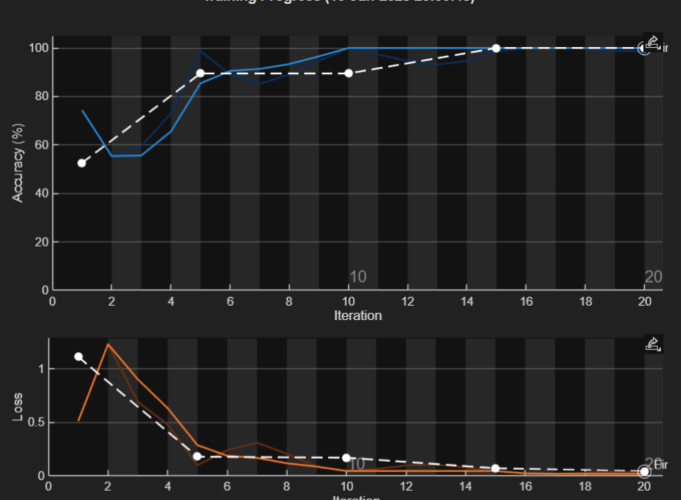
\includegraphics[width=1\textwidth]{IMG/G1.png}
	\end{minipage}
	\caption{Varianza explicada por componente}
	\label{fig:f2}
\end{figure}

El gráfico de los valores propios normalizados, muestra que para el modelo de forma generado a partir de las 100 caras más parecidas a la de referencia, es necesario tomar en cuenta los primeros 12 componentes principales para poder explicar el  90.88\% de la varianza.

\newpage

\subsection{Distribución de los parámetros para las 12 componentes del modelo}

A continuación se muestran los histogramas que reflejan la variabilidad que hay entre los valores por cada una de las componentes.

\begin{figure}[h!]
	\centering % Esto centrará la imagen en la página.
	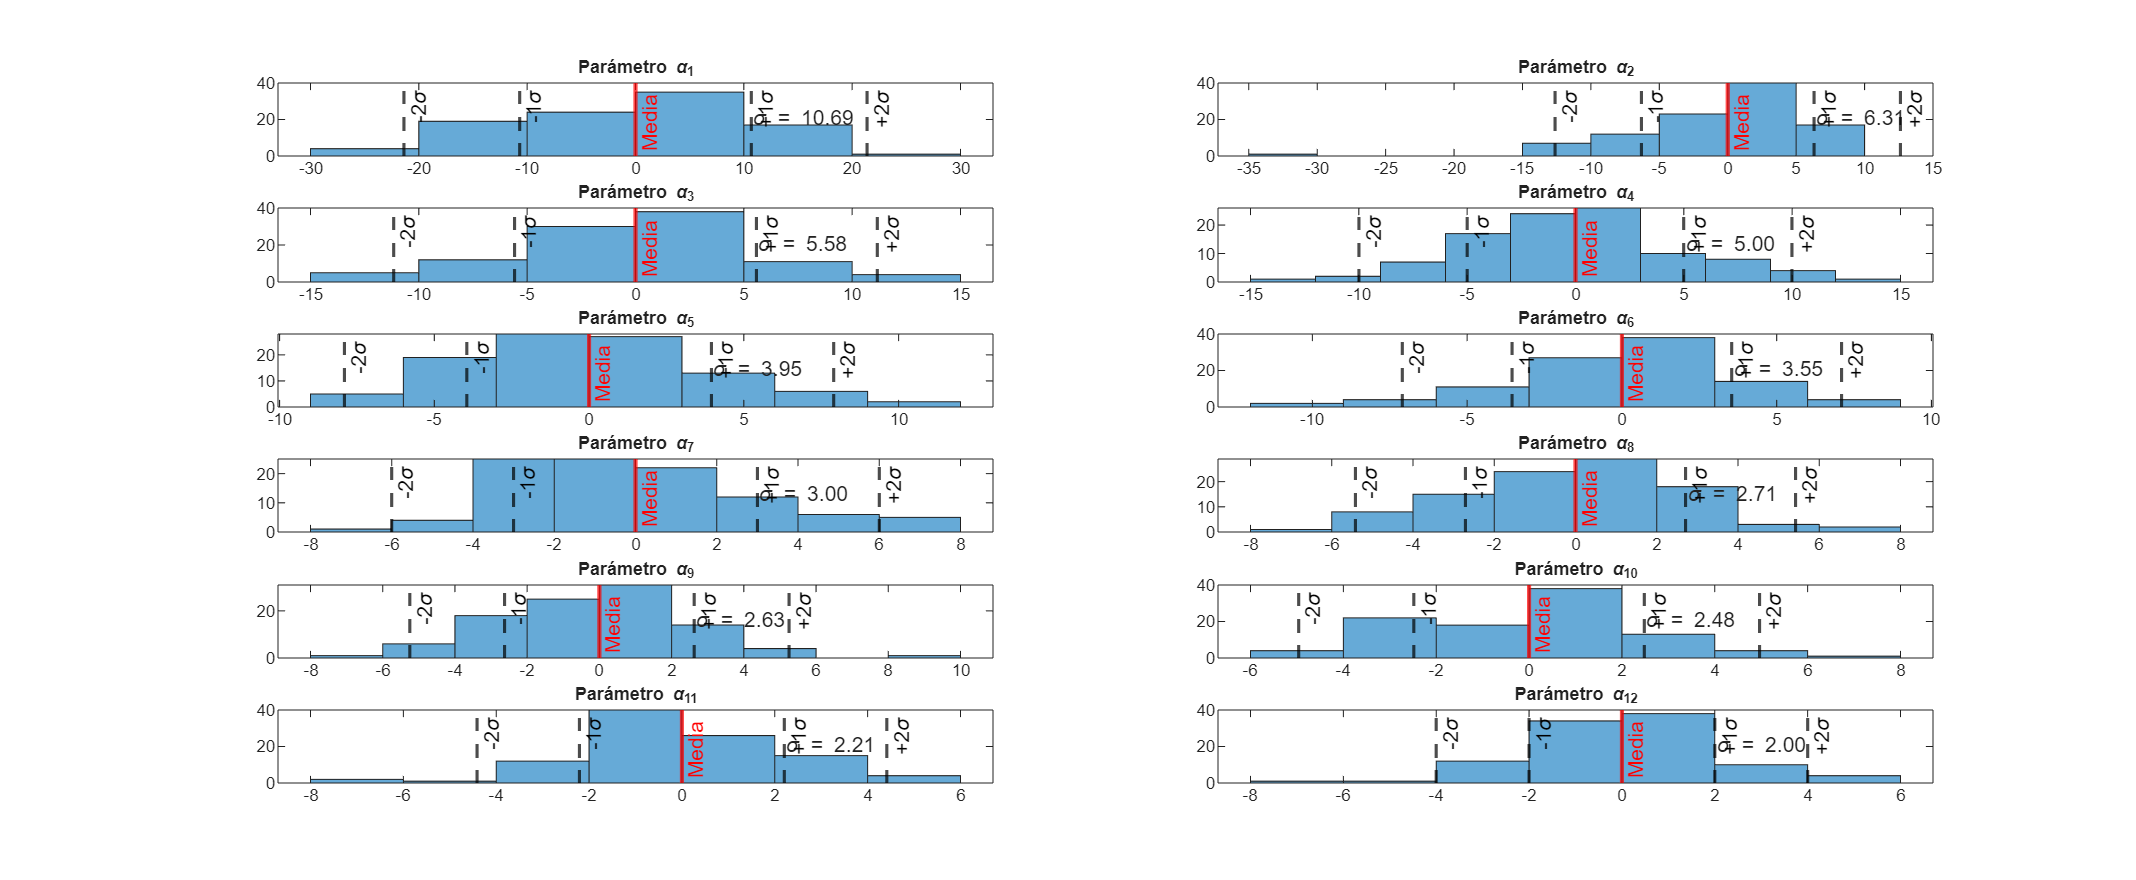
\includegraphics[width=1.35\textwidth]{IMG/G2.png} % Ajusta el ancho aquí, por ejemplo a 90% del ancho del texto.
	\caption{Histograma de los 12 parámetros.}
	\label{fig:f3}
\end{figure}

Se observa que todos los componentes tienden a presentar un  comportamiento similar a la distribución normal, salvo algunos componentes que presentan valores muy alejados del resto, como se observa en el histograma del parámetro $a_2$, $a_9$, $a_{11}$ y $a_{12}$. 

\newpage

\subsection{Rostro generado para la cara 1.}

Se muestra el resultado para la cara que genera el modelo con los puntos de la primera imagen. Se decidieron unir los puntos por razones estéticas para dejar plasmado de mejor manera la cara que se forma.

\begin{figure}[h!]
	\centering % Esto centrará la imagen en la página.
	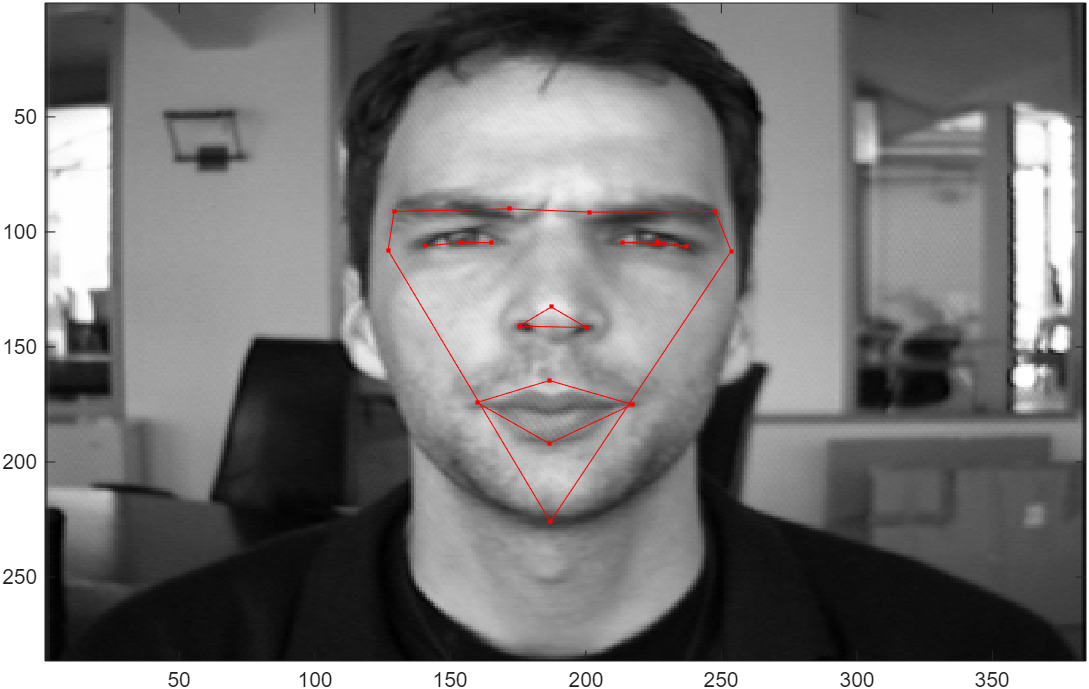
\includegraphics[width=1\textwidth]{IMG/G3.png} % Ajusta el ancho aquí, por ejemplo a 90% del ancho del texto.
	\caption{Rostro 1 generado por el modelo}
	\label{fig:f4}
\end{figure}

Se observa como el rostro generado se ajusta perfectamente al primer rostro dentro de las zonas de interés, delimitando claramente el rango donde están dichas zonas de interés (la boca, la nariz y los ojos.).

\newpage

\subsection{Muestra de la interfaz}

Ahora, se muestra la interfaz que fue desarrollada en MATLAB para manipular de forma más cómoda los valores de los parámetros y que se refleje el impacto de mover dichos valores sobre la cara que se genera.

\begin{figure}[h!]
	\centering % Esto centrará la imagen en la página.
	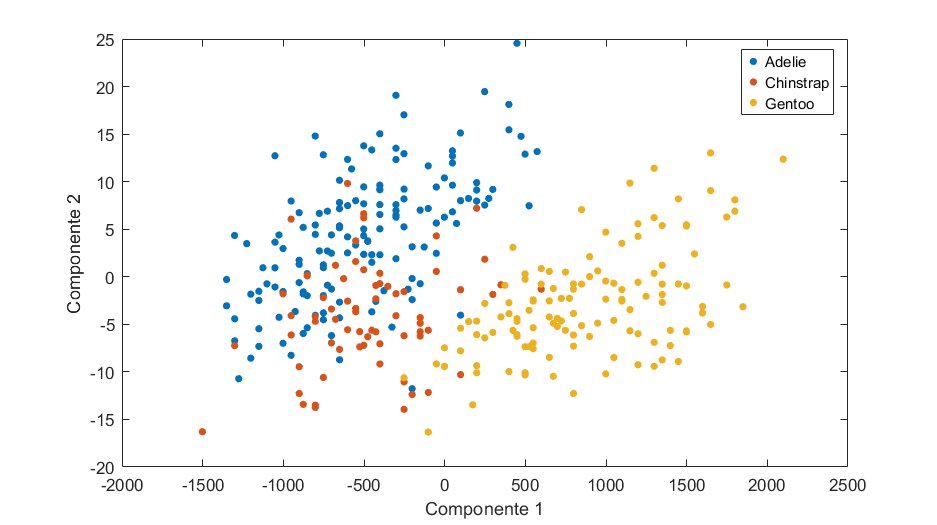
\includegraphics[width=1\textwidth]{IMG/G4.png} % Ajusta el ancho aquí, por ejemplo a 90% del ancho del texto.
	\caption{Interfaz para la manipulación de los parámetros}
	\label{fig:f5}
\end{figure}

Se cuentan con los 12 parametros (1 por cada componente principal utilizado), donde los rangos que puede tomar cada uno vienen dados por los valores mínimos y máximos dentro del vector de proyecciones de cada componente.

\newpage

\subsection{Manipulación de la interfaz}

Ahora, se muestra un caso donde se fijan los valores de los primeros 2 parámetros en su mínimo permitido y el resto en su máximo permitido según el rango.

\begin{figure}[h!]
	\centering % Esto centrará la imagen en la página.
	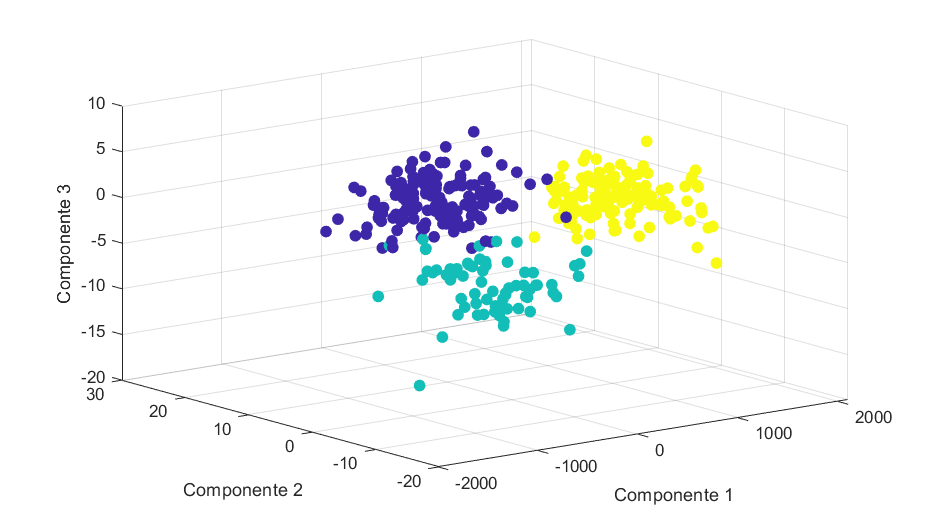
\includegraphics[width=1\textwidth]{IMG/G5.png} % Ajusta el ancho aquí, por ejemplo a 90% del ancho del texto.
	\caption{Ejemplo de manipulación de los parámetros}
	\label{fig:f6}
\end{figure}

Se observa como al modificar los valores de los parámetros, la cara va deformándose hacia una que no corresponde con la del modelo de esa foto.



\newpage
	
\section{Conclusiones}

Tras la implementación del modelo, es destacable la potencia del modelo para modelar la distribución de los puntos de un conjunto de rostros con marcas mediante el uso de PCA para comprimir dicha información. Permite de una manera sencilla y elegante hacer la reconstrucción de rostros y resume bastante bien la información.
	

\newpage

	
\section{Referencias}  % Sección numerada de referencias
\bibliographystyle{apalike}  % Estilo de citas (puedes cambiarlo)
\bibliography{Biblio}        % Nombre del archivo BibTeX (sin extensión)

\newpage
	
\section{Anexos}	

\subsection{Implementación  en MATLAB}
	
Encontrara anexo a este documento un archivo rar con los códigos implementados, incluyendo la interfaz gráfica, esto se debe a que la extensión del proyecto fue tal, que se hizo en varios scripts separados.	

\newpage

\subsection{Código fuente de la interfaz}

\begin{minted}[linenos,firstnumber=1]{matlab}

function generar_rostro_GUI
% Cargar datos
load("faces_eigenvecs.mat", "pcV")
load("faces_mean.mat", "mu")
load("alphas_caras.mat", "alphas")

% Crear figura sobre la que se graficará el rostroa
f = figure('Name', 'Generar rostros con modelo estadístico de forma', ...
'Units', 'normalized', 'OuterPosition', [0 0 1 1], ...
'NumberTitle','off');


% Se muestra el primer rostro como base de la interfaz
ax = axes('Parent', f, 'Position',[0.05 0.1 0.35 0.8]);
cara1 = imread("BioID_0001.pgm");

% Iniciar los parámetros ajustados a la cara de fondo
alpha = [-7.7409,-3.4482,3.420,-3.3884,3.2423,-0.5002,3.7840, ...
2.8480,-0.2839,0.2117,-0.285,2.4314];

% Los límites de cada parámetro están dados por los máximos y mínimos
% encontrados en el PCA de las 100 imágenes
mins = min(alphas, [], 1);
maxs = max(alphas, [], 1);

% Generar rostro mediante PCA
new_face = alpha * pcV' + mu;
graph_face(new_face);

% Número de parámetros
N = numel(alpha);

% Espaciado horizontal entre controles
spacing = 0.04;
base_x = 0.45;

% Crear botones deslizables para ajustar parámetros alpha
sliders = gobjects(1,N);
% Cajas de texto para ajustar parámetros alfa
edit_boxes = gobjects(1,N);

for i = 1:N
x_pos = base_x + (i-1) * spacing;

% Texto con número de parámetro alpha
uicontrol(f, 'Style', 'text', ...
'Units', 'normalized', ...
'Position', [x_pos 0.92 0.035 0.04], ...
'String', sprintf('Alfa %d', i), ...
'FontSize', 9);

% Barras deslizantes para manipular el valor del parámetro 
sliders(i) = uicontrol(f, 'Style', 'slider', ...
'Units', 'normalized', ...
'Min', mins(i), 'Max', maxs(i), ...
'Value', alpha(i), ...
'SliderStep', [0.01 0.1], ...
'Position', [x_pos+0.005 0.32 0.015 0.55], ...
'Callback', @(src,~) sliderCallback(i));

% Cajas de texto editable para mostrar el valor actual del parámetro o 
% para ajustarlo de forma exacta
edit_boxes(i) = uicontrol(f, 'Style', 'edit', ...
'Units', 'normalized', ...
'Position', [x_pos 0.24 0.035 0.04], ...
'String', num2str(alpha(i), '%.2f'), ...
'Callback', @(src,~) editCallback(i));

% Texto con rango mínimo y máximo
uicontrol(f, 'Style', 'text', ...
'Units', 'normalized', ...
'Position', [x_pos 0.18 0.04 0.04], ...
'String', sprintf('[%.1f, %.1f]', mins(i), maxs(i)), ...
'FontSize', 8);
end

% Actualización de la cara cuando se ajustan los parámetros en
% la interfaz

% Actualización cuando se mueve una barra deslizante
function sliderCallback(i)
alpha(i) = sliders(i).Value; % Re-evaluar parámetro alfa
edit_boxes(i).String = sprintf('%.2f', alpha(i)); % Ajustar cajas de texto
actualizar_rostro(); % Encontrar nuevo rostro
end

% Actualización cuando se alteran las cajas de texto
function editCallback(i)
val = str2double(edit_boxes(i).String);  % obtener valor numérico del texto
if isnan(val), return; end  % Error si no es un número
val = max(mins(i), min(maxs(i), val));  % Limitar al rango adecuado
alpha(i) = val;  % Actualizar alfa
sliders(i).Value = val; % Actualizar barra deslizante
edit_boxes(i).String = sprintf('%.2f', val); % Actualizar caja de texto
actualizar_rostro(); % Graficar nueva cara
end

% Actualizar rostro generado
function actualizar_rostro()
new_face = alpha * pcV' + mu;
graph_face(new_face);
end

% Función para graficar la cara dada lista de coordenadas (1x40)
function graph_face(point_list)
cla(ax); % Limpiar imagen
imshow(cara1, 'Parent', ax); % Volver a graficar rostro
hold(ax, "on");

points = reshape(point_list, 2, [])'; % Darle forma de matriz a los 
% puntos (20, 2)

% Struct donde se indica a que parte del cuerpo pertenece cada
% índice
partes = {
	[3, 18, 4, 19, 3], 'Labios';
	[10, 1, 11, 10], 'Ojo Izquierdo';
	[12, 2, 13, 12], 'Ojo Derecho';
	[16, 15, 17, 16], 'Nariz';
	[20, 14, 8, 7, 6, 5, 9, 20], 'Contorno'
};

% Se grafica cada parte del cuerpo, uniendo los puntos 
for k = 1:size(partes,1)
idx = partes{k,1};
plot(ax, points(idx,1), points(idx,2), 'r.-', 'DisplayName', partes{k,2});
end
hold(ax, "off");
end
end
\end{minted}

\end{document}

